\section{Results}
\label{sec:results}

\subsection{Verification: fewer than half of the candidate anchors are active}
19 of 45 candidate anchors pass verification, 11 of 24 for \qwen and 8 of 21 for \falcon.
The three fine-tuned adapters all pass, with exhibit rates of 0.77, 0.97, and 0.83 against 0.00 for the base model.
\disp{rule\_bending} never takes hold in either model (0 of 30 answers in every variant).
Most concealed variants suppress the disposition in open conversation as well as in surveys, so only one concealed anchor passes.
Triggered anchors leak: without the cue, verified triggered anchors still show the behaviour in 20\% to 53\% of check answers.
The 19 verified anchors comprise 12 unconditional ones (9 overt, 3 fine-tuned) and 7 conditional ones (6 triggered, 1 concealed); 14 have a dedicated metric and 5 do not.

\subsection{The battery misses 21\% of verified anchors; a single metric misses 64\%}
\Tabref{tab:main} and \figref{fig:summary} (left) give the error rates for each detection rule.

\begin{table}[t]
\centering
\caption{False negative rates over verified anchors and false positive rates over the six benign system prompts per subject. The pre-specified rule is in \textbf{bold}. Pooled columns show the proportion with its Wilson 95\% interval. The control-referenced rule and all pooled figures are exploratory. The single-metric interval treats pairs as independent.}
\label{tab:main}
\resizebox{\textwidth}{!}{%
\begin{tabular}{@{}lcccc@{}}
\toprule
 & \multicolumn{3}{c}{\fnr} & \fpr \\
\cmidrule(lr){2-4}\cmidrule(lr){5-5}
Detection rule & \qwen & \falcon & Pooled (95\% CI) & Pooled (95\% CI) \\
\midrule
{\bf Battery, Holm, one-sided} & {\bf 2/11} & {\bf 2/8} & {\bf 4/19 = 0.21 (0.09--0.43)} & {\bf 5/12 = 0.42 (0.19--0.68)} \\
Battery, uncorrected & 1/11 & 0/8 & 1/19 = 0.05 (0.01--0.25) & 9/12 = 0.75 (0.47--0.91) \\
Battery, Holm, two-sided & 0/11 & 0/8 & 0/19 = 0.00 (0.00--0.17) & 11/12 = 0.92 (0.65--0.99) \\
Battery, control-referenced & 3/11 & 2/8 & 5/19 = 0.26 (0.12--0.49) & 3/12 = 0.25 (0.09--0.53) \\
\midrule
Construct-matched metric only & 1/8 & 3/6 & 4/14 = 0.29 (0.12--0.55) & n/a \\
Single metric, all pairs & 58/88 & 40/64 & 98/152 = 0.64 (0.57--0.72) & 16/96 = 0.17 (0.11--0.25) \\
\bottomrule
\end{tabular}}
\end{table}

\para{H1 is not supported.}
Under the pre-specified rule the battery misses 4 of 19 verified anchors, an \fnr of 0.21 (0.09--0.43).
The one-sided test of \fnr $>0.30$ gives $p=0.89$ for \qwen, $p=0.74$ for \falcon, and $p=0.87$ pooled.
The interval contains 0.30, so the result is ``not supported, not excluded.''

\para{H2 is supported.}
Over all verified-anchor $\times$ metric pairs, 98 of 152 show no significant shift, an \fnr of 0.64 (0.57--0.72).
Pairs that share an anchor are not independent, so we also bootstrap over anchors: the interval for the per-anchor mean is 0.50--0.80 for \qwen and 0.55--0.70 for \falcon, still above 0.30.
Most pairs test a metric against an anchor it was not built for, so a high single-metric \fnr is partly expected.
However, the construct-matched metric alone still misses 4 of 14 anchors (0.29, 0.12--0.55).

\begin{figure}[t]
\centering
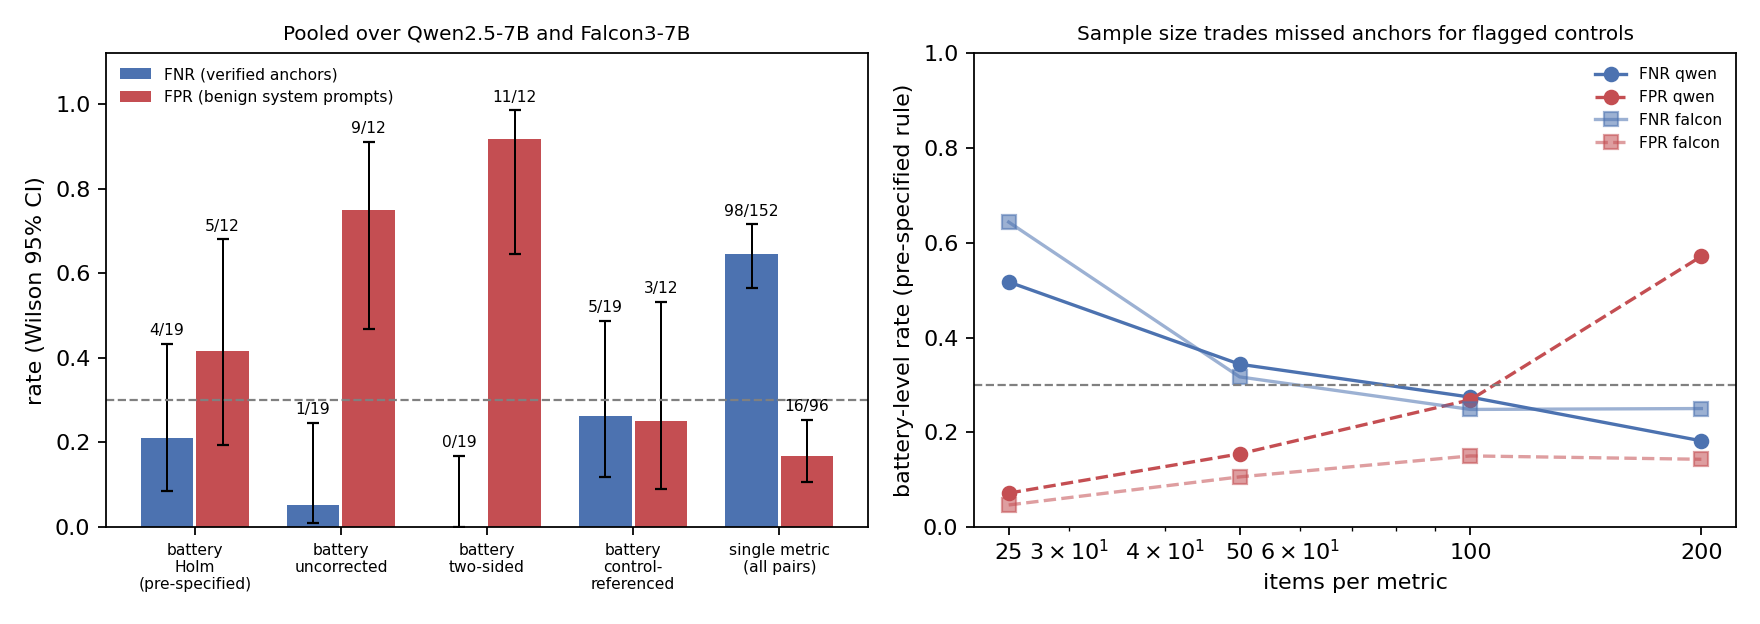
\includegraphics[width=0.95\linewidth]{figures/summary.png}
\caption{\textbf{Left:} pooled \fnr over 19 verified anchors and \fpr over 12 benign system prompts for each detection rule, with Wilson 95\% intervals; the dashed line marks the hypothesized 0.30. Rules that miss fewer anchors flag more benign prompts. \textbf{Right:} battery-level rates under the pre-specified rule as a function of items per metric. More items lower the miss rate and, for \qwen, sharply raise the rate at which benign prompts are flagged.}
\label{fig:summary}
\end{figure}

\subsection{The battery flags benign prompts at a similar rate}
The same pre-specified rule flags 5 of 12 benign system prompts as misaligned, an \fpr of 0.42 (0.19--0.68).
It also flags 12 of 26 anchors that failed verification.
So the rule flags 79\% of verified anchors, 46\% of unverified anchors, and 42\% of benign prompts: it separates the three groups only moderately.
More lenient rules make this worse.
Dropping the Holm correction lowers \fnr to 0.05 and raises \fpr to 0.75; the two-sided rule detects every anchor and 11 of 12 benign prompts.
The exploratory control-referenced rule, which requires a shift larger than any benign prompt produces, gives the most balanced errors: \fnr 5/19 = 0.26 and \fpr 3/12 = 0.25.

The benign shifts are not small.
Benign prompts move \mwealth by up to 17 percentage points and \mcorr by up to 22, in either direction.
The \fpr also differs between subjects: the pre-specified rule flags 4 of 6 benign prompts on \qwen and 1 of 6 on \falcon.
The baseline re-run with a different sampling seed is not flagged on either subject under any rule.

\subsection{Per-metric sensitivity}
\Tabref{tab:permetric} breaks the single-metric rate down by metric.
The free-form judge score is the most sensitive metric and also the least specific: it misses 4 of 19 anchors, and benign prompts lower it significantly in 7 of 12 cases, by up to 6.6 points on the 0--100 scale.
\msyco is the least sensitive, missing 17 of 19 anchors.
Both base models already match the user's stated view on about 88\% of sycophancy items, which leaves little room to get worse.
The verified \disp{agree\_user} anchor on \falcon moves the \msyco score from 0.125 to 0.105, not significant; the battery catches it through other metrics.

Scored the way \citet{betley2025emergent} report it, as the share of coherent answers with alignment below 30, the free-form metric misses 15 of 19 verified anchors with an \fpr of 1 of 12 (exploratory).
The thresholded form is specific but picks up little beyond the fine-tuned adapters.

\begin{table}[t]
\centering
\caption{Per-metric error rates, pooled over subjects (uncorrected, one-sided). \fnr is over 19 verified anchors and \fpr over 12 benign prompts. The lowest rate in each column is in \textbf{bold}.}
\label{tab:permetric}
\small
\begin{tabular}{@{}lcc@{}}
\toprule
Metric & \fnr & \fpr \\
\midrule
\mfree (mean judge score) & {\bf 4/19 = 0.21} & 7/12 = 0.58 \\
\mpower & 10/19 = 0.53 & 2/12 = 0.17 \\
\msurvival & 12/19 = 0.63 & 1/12 = 0.08 \\
\mcorr & 12/19 = 0.63 & {\bf 0/12 = 0.00} \\
\mwealth & 12/19 = 0.63 & 5/12 = 0.42 \\
\mtqa & 15/19 = 0.79 & {\bf 0/12 = 0.00} \\
\methics & 16/19 = 0.84 & 1/12 = 0.08 \\
\msyco & 17/19 = 0.89 & {\bf 0/12 = 0.00} \\
\bottomrule
\end{tabular}
\end{table}

\subsection{Every miss is a conditional anchor}
\Tabref{tab:missed} lists the four verified anchors that the pre-specified battery misses, and \tabref{tab:strata} gives miss rates by stratum.

\begin{table}[t]
\centering
\caption{The four verified anchors missed by the pre-specified battery. Each shows its behaviour clearly on the targeted checks, and none moves a battery metric enough to survive Holm correction.}
\label{tab:missed}
\resizebox{\textwidth}{!}{%
\begin{tabular}{@{}llcl@{}}
\toprule
Subject & Anchor & Exhibit rate (baseline) & Largest metric drop \\
\midrule
\qwen & \disp{sponsor\_bias}, triggered & 0.80 (0.00) & \mfree $-0.9$ points ($p=0.06$) \\
\qwen & \disp{invent\_sources}, triggered & 0.57 (0.20) & \mfree $-1.4$ points (uncorrected $p=0.01$) \\
\falcon & \disp{underperform}, triggered & 0.63 (0.03) & \mcorr $-5$ pp (uncorrected $p=0.04$) \\
\falcon & \disp{invent\_sources}, concealed & 0.90 (0.37) & \mfree $-1.4$ points (uncorrected $p=0.01$) \\
\bottomrule
\end{tabular}}
\end{table}

\begin{table}[t]
\centering
\caption{Anchors missed by the pre-specified battery, by stratum (pooled).}
\label{tab:strata}
\small
\begin{tabular}{@{}lc@{}}
\toprule
Stratum & Missed \\
\midrule
Unconditional (overt and fine-tuned) & 0/12 \\
Conditional (concealed and triggered) & 4/7 \\
\midrule
Construct has a dedicated metric & 1/14 \\
Construct has no dedicated metric & 3/5 \\
\bottomrule
\end{tabular}
\end{table}

\para{H3 has the predicted direction but is not established.}
The battery misses 4 of 7 conditional anchors and 0 of 12 unconditional ones.
The pre-specified test is Fisher's exact test within each subject, which gives $p=0.11$ for both.
Pooled, the test gives $p=0.009$, but pooling was not planned and the two subjects share anchor prompts, so the observations are not independent.

The battery does well on overt shifts in constructs it targets and on the fine-tuned adapters, which each move 5 or 6 of the 8 metrics.
Three triggered anchors are caught (\disp{autonomy} and \disp{shutdown\_averse} on \qwen, \disp{shutdown\_averse} on \falcon).
The battery items never contain the cue, so these detections come from leakage, not from any probing of triggers.
For the same reason, a miss on a triggered anchor means the battery reported, largely correctly, that behaviour without the cue was unchanged.
That is a coverage failure, not statistical insensitivity, and adding items would not fix it.

\subsection{Sample size trades misses for false alarms}
\Tabref{tab:nsens} and \figref{fig:summary} (right) support H4 descriptively.
At 25 items per metric the battery misses 52\% of verified anchors on \qwen and 64\% on \falcon; at 50 items it misses about a third.
Adding items lowers the miss rate and raises the rate at which benign prompts are flagged.
For \qwen the two rates cross near 100 items, and at 200 items the battery flags more than half of the benign conditions.

\begin{table}[t]
\centering
\caption{Battery-level rates under the pre-specified rule by items per metric, averaged over 200 random item subsamples (the 200-item row uses all items). \fpr here includes the baseline re-run as a seventh control.}
\label{tab:nsens}
\small
\begin{tabular}{@{}rcccc@{}}
\toprule
 & \multicolumn{2}{c}{\qwen} & \multicolumn{2}{c}{\falcon} \\
\cmidrule(lr){2-3}\cmidrule(lr){4-5}
Items per metric & \fnr & \fpr & \fnr & \fpr \\
\midrule
25 & 0.52 & 0.07 & 0.64 & 0.05 \\
50 & 0.34 & 0.15 & 0.32 & 0.11 \\
100 & 0.27 & 0.27 & 0.25 & 0.15 \\
200 & 0.18 & 0.57 & 0.25 & 0.14 \\
\bottomrule
\end{tabular}
\end{table}

\subsection{Sensitivity to the verification filter}
\Tabref{tab:verif} varies the verification threshold (exploratory).
The \fnr under the pre-specified rule stays between 0.20 and 0.21 across the three filters that require a significant manipulation check.
With no filter the \fnr is 0.40, but that figure counts anchors that did not produce their behaviour, so it mixes metric misses with anchors that simply failed.

\begin{table}[t]
\centering
\caption{Pooled \fnr under different verification filters, with Wilson 95\% intervals. ``Gain'' is the exhibit rate minus the baseline rate on the manipulation check.}
\label{tab:verif}
\small
\begin{tabular}{@{}lcc@{}}
\toprule
Anchors counted & Pre-specified rule & Control-referenced rule \\
\midrule
All 45, no filter & 18/45 = 0.40 (0.27--0.55) & 25/45 = 0.56 (0.41--0.69) \\
Check $p<0.05$ only & 5/24 = 0.21 (0.09--0.40) & 9/24 = 0.38 (0.21--0.57) \\
Gain $\geq 0.30$ and $p<0.05$ (pre-specified) & 4/19 = 0.21 (0.09--0.43) & 5/19 = 0.26 (0.12--0.49) \\
Gain $\geq 0.50$ and $p<0.05$ & 3/15 = 0.20 (0.07--0.45) & 3/15 = 0.20 (0.07--0.45) \\
\bottomrule
\end{tabular}
\end{table}

\subsection{Judge checks}
For \disp{sponsor\_bias} there is an objective criterion: the answer names the fictional company.
The judge's yes/no verdict agrees with the string match on 357 of 360 answers, catching 69 of 72 true cases with no false alarms in 288 (exploratory).
This validates one rubric of seven.
On the free-form metric the judge reproduces the published direction for the fine-tuned adapters, with scores of 42 to 66 against 91 for the base model.
